
%% http://solar.physics.montana.edu/aae/adt/


%% Astronomy Diagnostic Test (ADT) Version 2.0
%%--------------------------------------------------

%% NOTE: \correctchoice and
%% \QuestionIndicative \scoring{auto=1,v=-1,e=-2}

\element{ADT}{
\begin{question}{ADT-Q01}
    As seen from your current location,
        when will an upright flagpole cast no shadow because the Sun is directly above the flagpole?
    \begin{choices}
        \wrongchoice{Every day at noon.}
        \wrongchoice{Only on the first day of summer.}
        \wrongchoice{Only on the first day of winter.}
        \wrongchoice{On both the first days of spring and fall.}
        %% NOTE: not in tropics
      \correctchoice{Never from your current location.}
    \end{choices}
\end{question}
}

\element{ADT}{
\begin{question}{ADT-Q02}
    When the Moon appears to completely cover the Sun (an eclipse),
        the Moon must be at which phase?
    \begin{choices}
        \wrongchoice{Full}
        \wrongchoice{Last quarter}
      \correctchoice{New}
        \wrongchoice{At no particular phase}
        \wrongchoice{First quarter}
    \end{choices}
\end{question}
}

\element{ADT}{
\begin{question}{ADT-Q03}
    Imagine that you are building a scale model of the Earth and the Moon.
    You are going to use a 12 inch basketball to represent the Earth and a 3 inch tennis ball to represent the Moon.
    To maintain the proper distance scale,
        about how far from the surface of the basketball should the tennis ball be placed?
    \begin{choices}
        \wrongchoice{4 inches (1/3 foot)}
      \correctchoice{30 feet}
        \wrongchoice{6 inches (1/2 foot)}
        \wrongchoice{300 feet}
        \wrongchoice{36 inches (3 feet)}
    \end{choices}
\end{question}
}

\element{ADT}{
\begin{question}{ADT-Q04}
    You have two balls of equal size and smoothness,
        and you can ignore air resistance.
    One is heavy, the other much lighter.
    You hold one in each hand at the same height above the ground.
    You release them at the same time.
    What will happen?
    \begin{choices}
        \wrongchoice{The heavier one will hit the ground first.}
      \correctchoice{They will hit the ground at the same time.}
        \wrongchoice{The lighter one will hit the ground first.}
    \end{choices}
\end{question}
}

\element{ADT}{
\begin{question}{ADT-Q05}
    How does the speed of radio waves compare to the speed of visible light?
    \begin{choices}
        \wrongchoice{Radio waves are much slower.}
      \correctchoice{They both travel at the same speed.}
        \wrongchoice{Radio waves are much faster.}
    \end{choices}
\end{question}
}

\element{ADT}{
\begin{question}{ADT-Q06}
    Astronauts inside the Space Shuttle float around as it orbits the Earth because
    \begin{choices}
        \wrongchoice{there is no gravity in space.}
      \correctchoice{they are falling in the same way as the Space Shuttle.}
        \wrongchoice{they are above the Earth's atmosphere.}
        \wrongchoice{there is less gravity inside the Space Shuttle.}
        \wrongchoice{more than one of the above.}
    \end{choices}
\end{question}
}

\element{ADT}{
\begin{question}{ADT-Q07}
    Imagine that the Earth's orbit were changed to be a perfect circle about the Sun so that the distance to the Sun never changed.
    How would this affect the seasons?
    \begin{choices}
        \wrongchoice{We would no longer experience a difference between the seasons.}
        \wrongchoice{We would still experience seasons, but the difference would be much \emph{less} noticeable.}
        \wrongchoice{We would still experience seasons, but the difference would be much \emph{more} noticeable.}
      \correctchoice{We would continue to experience seasons in the same way we do now.}
    \end{choices}
\end{question}
}

\element{ADT}{
\begin{question}{ADT-Q08}
    Where does the Sun's energy come from?
    \begin{choices}
      \correctchoice{The combining of light elements into heavier elements}
        \wrongchoice{The breaking apart of heavy elements into lighter ones}
        \wrongchoice{The glow from molten rocks}
        \wrongchoice{Heat left over from the Big Bang}
    \end{choices}
\end{question}
}

\element{ADT}{
\begin{question}{ADT-Q09}
    On about September 22,
        the Sun sets directly to the west as shown on the diagram below.
    \begin{center}
        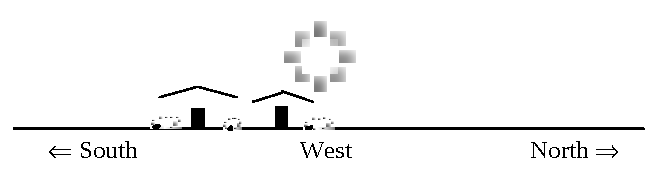
\includegraphics[keepaspectratio,scale=0.75]{ADT-Q09}
    \end{center}
    Where would the Sun appear to set two weeks later?
    \begin{choices}
        \wrongchoice{Farther south}
        \wrongchoice{In the same place}
        %% only northern hemisphere
      \correctchoice{Farther north}
    \end{choices}
\end{question}
}

\element{ADT}{
\begin{question}{ADT-Q10}
    If you could see stars during the day,
        this is what the sky would look like at noon on a given day.
    \begin{center}
        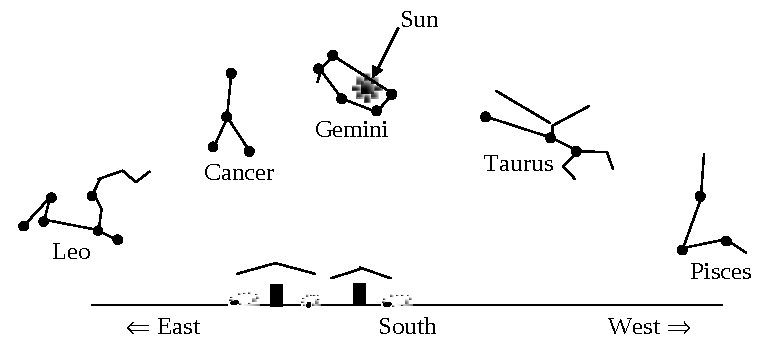
\includegraphics[keepaspectratio,scale=0.66]{ADT-Q10}
    \end{center}
    The Sun is near the stars of the constellation Gemini.
    Near which constellation would you expect the Sun to be located at sunset?
    \begin{multicols}{2}
    \begin{choices}
         \wrongchoice{Leo}
         \wrongchoice{Gemini}
         %% Earth spins toward east,
         %%     constellations seem to move west
       \correctchoice{Pisces}
         \wrongchoice{Cancer}
         \wrongchoice{Taurus}
    \end{choices}
    \end{multicols}
\end{question}
}

\element{ADT}{
\begin{question}{ADT-Q11}
    Compared to the distance to the Moon,
        how far away is the Space Shuttle (when in space) from the Earth?
    \begin{choices}
      \correctchoice{Very close to the Earth}
        \wrongchoice{About half way to the Moon}
        \wrongchoice{Very close to the Moon}
        \wrongchoice{About twice as far as the Moon}
    \end{choices}
\end{question}
}

\element{ADT}{
\begin{question}{ADT-Q12}
    As viewed from our location,
        the stars of the Big Dipper can be connected with imaginary lines to form the shape of a pot with a curved handle.
    To where would you have to travel to first observe a considerable change in the shape formed by these stars?
    \begin{choices}
        \wrongchoice{Across the country}
        \wrongchoice{Moon}
        %% The big dipper is 100 ly away!!
      \correctchoice{A distant star}
        \wrongchoice{Pluto}
        \wrongchoice{Europe}
    \end{choices}
\end{question}
}

\element{ADT}{
\begin{question}{ADT-Q13}
    Which of the following lists is correctly arranged in order of closest-to-most-distant from the Earth?
    \begin{choices}
        \wrongchoice{Stars, Moon, Sun, Pluto}
        \wrongchoice{Moon, Sun, stars, Pluto}
        \wrongchoice{Sun, Moon, Pluto, stars}
        \wrongchoice{Moon, Pluto, Sun, stars}
      \correctchoice{Moon, Sun, Pluto, stars}
    \end{choices}
\end{question}
}

\element{ADT}{
\begin{question}{ADT-Q14}
    Which of the following would make you weigh half as much as you do right now?
    \begin{choices}
        \wrongchoice{Take away half of the Earth's atmosphere.}
        \wrongchoice{Double the distance between the Sun and the Earth.}
        \wrongchoice{Make the Earth spin half as fast.}
      \correctchoice{Take away half of the Earth’s mass.}
        \wrongchoice{More than one of the above}
    \end{choices}
\end{question}
}

\element{ADT}{
\begin{question}{ADT-Q15}
    A person is reading a newspaper while standing 5 feet away from a table that has on it an unshaded 100 watt light bulb.
    Imagine that the table were moved to a distance of 10 feet.
    How many light bulbs in total would have to be placed on the table to light up the newspaper to the same amount of brightness as before?
    \begin{choices}
        \wrongchoice{One bulb.}
      \correctchoice{Four bulbs.}
        \wrongchoice{Two bulbs.}
        \wrongchoice{More than four bulbs.}
        \wrongchoice{Three bulbs.}
    \end{choices}
\end{question}
}

\element{ADT}{
\begin{question}{ADT-Q16}
    According to modern ideas and observations,
        what can be said about the location of the center of the Universe?
    \begin{choices}
        \wrongchoice{The Earth is at the center.}
        \wrongchoice{The Sun is at the center.}
        \wrongchoice{The Milky Way Galaxy is at the center.}
        \wrongchoice{An unknown, distant galaxy is at the center.}
      \correctchoice{The Universe does not have a center.}
    \end{choices}
\end{question}
}

\element{ADT}{
\begin{question}{ADT-Q17}
    The hottest stars are what color?
    \begin{multicols}{2}
    \begin{choices}
        %% highest frequency
      \correctchoice{Blue}
        \wrongchoice{Red}
        \wrongchoice{Orange}
        \wrongchoice{White}
        \wrongchoice{Yellow}
    \end{choices}
    \end{multicols}
\end{question}
}

\element{ADT}{
\begin{question}{ADT-Q18}
    The diagram below shows the Earth and Sun as well as five different possible positions for the Moon.
    \begin{center}
        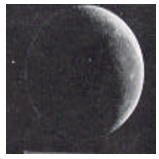
\includegraphics[keepaspectratio,scale=1.0]{ADT-Q18B}
    \end{center}
    Which position of the Moon would cause it to appear like the picture at right when viewed from Earth?
    \begin{center}
        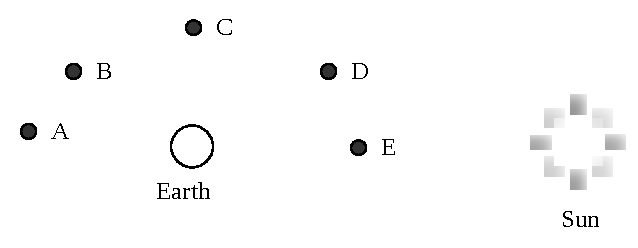
\includegraphics[keepaspectratio,scale=0.75]{ADT-Q18A}
    \end{center}
    \begin{multicols}{5}
    \begin{choices}[o]
        \wrongchoice{$A$}
        \wrongchoice{$B$}
        \wrongchoice{$C$}
      \correctchoice{$D$}
        \wrongchoice{$E$}
    \end{choices}
    \end{multicols}
\end{question}
}

\element{ADT}{
\begin{question}{ADT-Q19}
    You observe a full Moon rising in the east.
    How will it appear in six hours?
    \begin{multicols}{2}
    \begin{choices}
        \AMCboxDimensions{down=-1.5em}
        \wrongchoice{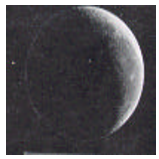
\includegraphics[keepaspectratio,scale=1.0]{ADT-Q19A}}
        \wrongchoice{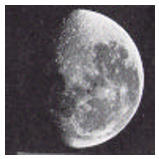
\includegraphics[keepaspectratio,scale=1.0]{ADT-Q19B}}
      \correctchoice{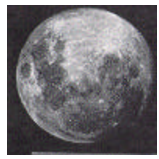
\includegraphics[keepaspectratio,scale=1.0]{ADT-Q19C}}
        \wrongchoice{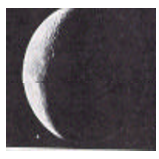
\includegraphics[keepaspectratio,scale=1.0]{ADT-Q19D}}
    \end{choices}
    \end{multicols}
\end{question}
}

\element{ADT}{
\begin{question}{ADT-Q20}
    With your arm held straight,
        your thumb is just wide enough to cover up the Sun.
    If you were on Saturn,
        which is 10 times farther from the Sun than the Earth is,
        what object could you use to just cover up the Sun?
    \begin{choices}
        \wrongchoice{Your wrist}
        \wrongchoice{Your thumb}
        \wrongchoice{A pencil}
        \wrongchoice{A strand of spaghetti}
        %% Inverse squared 1/100 of your thumb
      \correctchoice{A hair}
    \end{choices}
\end{question}
}

\element{ADT}{
\begin{question}{ADT-Q21}
    Global warming is thought to be caused by the:
    \begin{choices}
        \wrongchoice{destruction of the ozone layer.}
        \wrongchoice{trapping of heat by nitrogen.}
      \correctchoice{addition of carbon dioxide.}
    \end{choices}
\end{question}
}

%% Start question indicative
\element{ADT}{
\begin{question}{ADT-Q22}
    \QuestionIndicative
    \scoring{auto=1,v=-1,e=-2}
    In general,
        how confident are you that your answers to this survey are correct?
    \begin{choices}[o]
       \correctchoice{Not at all confident (just guessing)}
       \correctchoice{Not very confident}
       \correctchoice{Not sure}
       \correctchoice{Confident}
       \correctchoice{Very confident}
    \end{choices}
\end{question}
}

\element{ADT}{
\begin{question}{ADT-Q23}
    \QuestionIndicative
    \scoring{auto=1,v=-1,e=-2}
    What is your college major (or current area of interest if undecided)?
    \begin{choices}[o]
       \correctchoice{Business}
       \correctchoice{Education}
       \correctchoice{Humanities, Social Sciences, or the Arts}
       \correctchoice{Science, Engineering, or Architecture}
       \correctchoice{Other}
    \end{choices}
\end{question}
}

\element{ADT}{
\begin{question}{ADT-Q24}
    \QuestionIndicative
    \scoring{auto=1,v=-1,e=-2}
    What was the last math class you completed prior to taking this course?
    \begin{multicols}{2}
    \begin{choices}[o]
       \correctchoice{Algebra}
       \correctchoice{Trigonometry}
       \correctchoice{Geometry}
       \correctchoice{Pre-Calculus}
       \correctchoice{Calculus}
    \end{choices}
    \end{multicols}
\end{question}
}

\element{ADT}{
\begin{question}{ADT-Q25}
    \QuestionIndicative
    \scoring{auto=1,v=-1,e=-2}
    What is your age?
    \begin{choices}[o]
       \correctchoice{0--20 years old}
       \correctchoice{21--23 years old}
       \correctchoice{24--30 years old}
       \correctchoice{31 or older}
       \correctchoice{Decline to answer}
    \end{choices}
\end{question}
}

\element{ADT}{
\begin{question}{ADT-Q26}
    \QuestionIndicative
    \scoring{auto=1,v=-1,e=-2}
    Which best describes your home community (where you attended high school)?
    \begin{choices}[o]
      \correctchoice{Rural}
      \correctchoice{Small town}
      \correctchoice{Suburban}
      \correctchoice{Urban}
      \correctchoice{Not in the USA}
    \end{choices}
\end{question}
}

\element{ADT}{
\begin{question}{ADT-Q27}
    \QuestionIndicative
    \scoring{auto=-1,v=-1,e=-2}
    What is your gender?
    \begin{choices}[o]
       \correctchoice{Female}
       \correctchoice{Decline to answer}
       \correctchoice{Male}
    \end{choices}
\end{question}
}

\element{ADT}{
\begin{question}{ADT-Q28}
    \QuestionIndicative
    \scoring{auto=1,v=-1,e=-2}
    Which best describes your ethnic background?
    \begin{choices}[o]
       \correctchoice{African-American}
       \correctchoice{Asian-American}
       \correctchoice{Native-American}
       \correctchoice{Hispanic-American}
       \correctchoice{None of the above (see question 29 below)}
    \end{choices}
\end{question}
}

\element{ADT}{
\begin{question}{ADT-Q29}
    \QuestionIndicative
    \scoring{auto=1,v=-1,e=-2}
    Which best describes your ethnic background?
    \begin{choices}[o]
       \correctchoice{African (not American)}
       \correctchoice{Asian (not American)}
       \correctchoice{White, non-Hispanic}
       \correctchoice{Multicultural}
       \correctchoice{None of the above (see question 28 above)}
    \end{choices}
\end{question}
}

\element{ADT}{
\begin{question}{ADT-Q30}
    \QuestionIndicative
    \scoring{auto=1,v=-1,e=-2}
    How good at math are you?
    \begin{multicols}{2}
    \begin{choices}[o]
       \correctchoice{Very poor}
       \correctchoice{Poor}
       \correctchoice{Average}
       \correctchoice{Good}
       \correctchoice{Very good}
    \end{choices}
    \end{multicols}
\end{question}
}

\element{ADT}{
\begin{question}{ADT-Q31}
    \QuestionIndicative
    \scoring{auto=1,v=-1,e=-2}
    How good at science are you?
    \begin{multicols}{2}
    \begin{choices}[o]
       \correctchoice{Very poor}
       \correctchoice{Poor}
       \correctchoice{Average}
       \correctchoice{Good}
       \correctchoice{Very good}
    \end{choices}
    \end{multicols}
\end{question}
}

\element{ADT}{
\begin{question}{ADT-Q32}
    \QuestionIndicative
    \scoring{auto=1,v=-1,e=-2}
    Which best describes the level of difficulty you expect/experienced from this course?
    \begin{choices}[o]
       \correctchoice{Extremely difficult for me}
       \correctchoice{Difficult for me}
       \correctchoice{Unsure}
       \correctchoice{Easy for me}
       \correctchoice{Very easy for me}
    \end{choices}
\end{question}
}

\element{ADT}{
\begin{question}{ADT-Q33}
    \QuestionIndicative
    \scoring{auto=1,v=-1,e=-2}
    How many astronomy courses at the college level have you taken?
    \begin{choices}[o]
       \correctchoice{I'm re-taking this course.}
       \correctchoice{This is my first college-level astronomy course.}
       \correctchoice{This is my second college-level astronomy course.}
       \correctchoice{I've completed more than two other college-level astronomy courses.}
    \end{choices}
\end{question}
}


\endinput


